\chapter{Đánh giá so sánh với các bài báo khác giải quyết cùng vấn đề.}
\section{Bitcoin Price Prediction and Analysis Using Deep Learning Models}
\subsection{Giới thiệu bài báo}
Bài báo được viết bởi Awoke et al. \cite{5} và xuất bản vào năm 2021, tập trung vào việc ứng dụng các mô hình học sâu để dự đoán giá Bitcoin. Mục tiêu của nghiên cứu này là áp dụng các mô hình học sâu cơ bản, cụ thể là \textit{Long Short-Term Memory} (LSTM) và \textit{Gated Recurrent Unit} (GRU), để dự đoán giá Bitcoin. Bài báo của Awoke et al. (2021) đã so sánh hiệu quả của hai mô hình này bằng cách sử dụng các chỉ số lỗi như \textit{Root Mean Squared Error} (RMSE) và \textit{Mean Absolute Percentage Error} (MAPE).

Bài báo sử dụng mô hình LSTM và GRU cơ bản với cấu hình truyền thống mà không tinh chỉnh nhiều yếu tố khác. Do đó việc so sánh kết quả bài báo này là quan trọng để thấy được mô hình LSTM và Random Forest mà chúng tôi đã cung cấp ở trên có độ chính xác thế nào so với việc áp dụng một mô hình học sâu truyền thống.
\subsection{Bộ dữ liệu}
Dữ liệu được thu thập từ trang \textit{Kaggle}, bao gồm giá trị mở cửa, giá cao nhất, giá thấp nhất, giá đóng cửa, và vốn hóa thị trường của Bitcoin từ 1/1/2014 đến 20/2/2018. Bộ dữ liệu đã được chuẩn bị và chuẩn hóa để phù hợp với việc huấn luyện mô hình.
\subsection{Phương pháp}
Tác giả đã sử dụng các mô hình học sâu cơ bản (basic deep learning-based models), cụ thể là mô hình LSTM và GRU được sử dụng với cấu hình truyền thống mà không tinh chỉnh nhiều yếu tố khác. Điều này có nghĩa là họ chỉ so sánh các mô hình học sâu cơ bản để xem xét hiệu suất dự đoán của chúng đối với giá Bitcoin.

Mô hình LSTM và GRU được sử dụng vì chúng có khả năng xử lý tốt các phụ thuộc dài hạn trong chuỗi thời gian. Hai mô hình này được huấn luyện với số lượng \textit{epoch} là 100 và sử dụng bộ \textit{batch size} là 32. Mục tiêu là dự đoán giá Bitcoin cho các ngày tiếp theo và so sánh kết quả của hai mô hình.

\begin{figure}[h!]
    \centering
    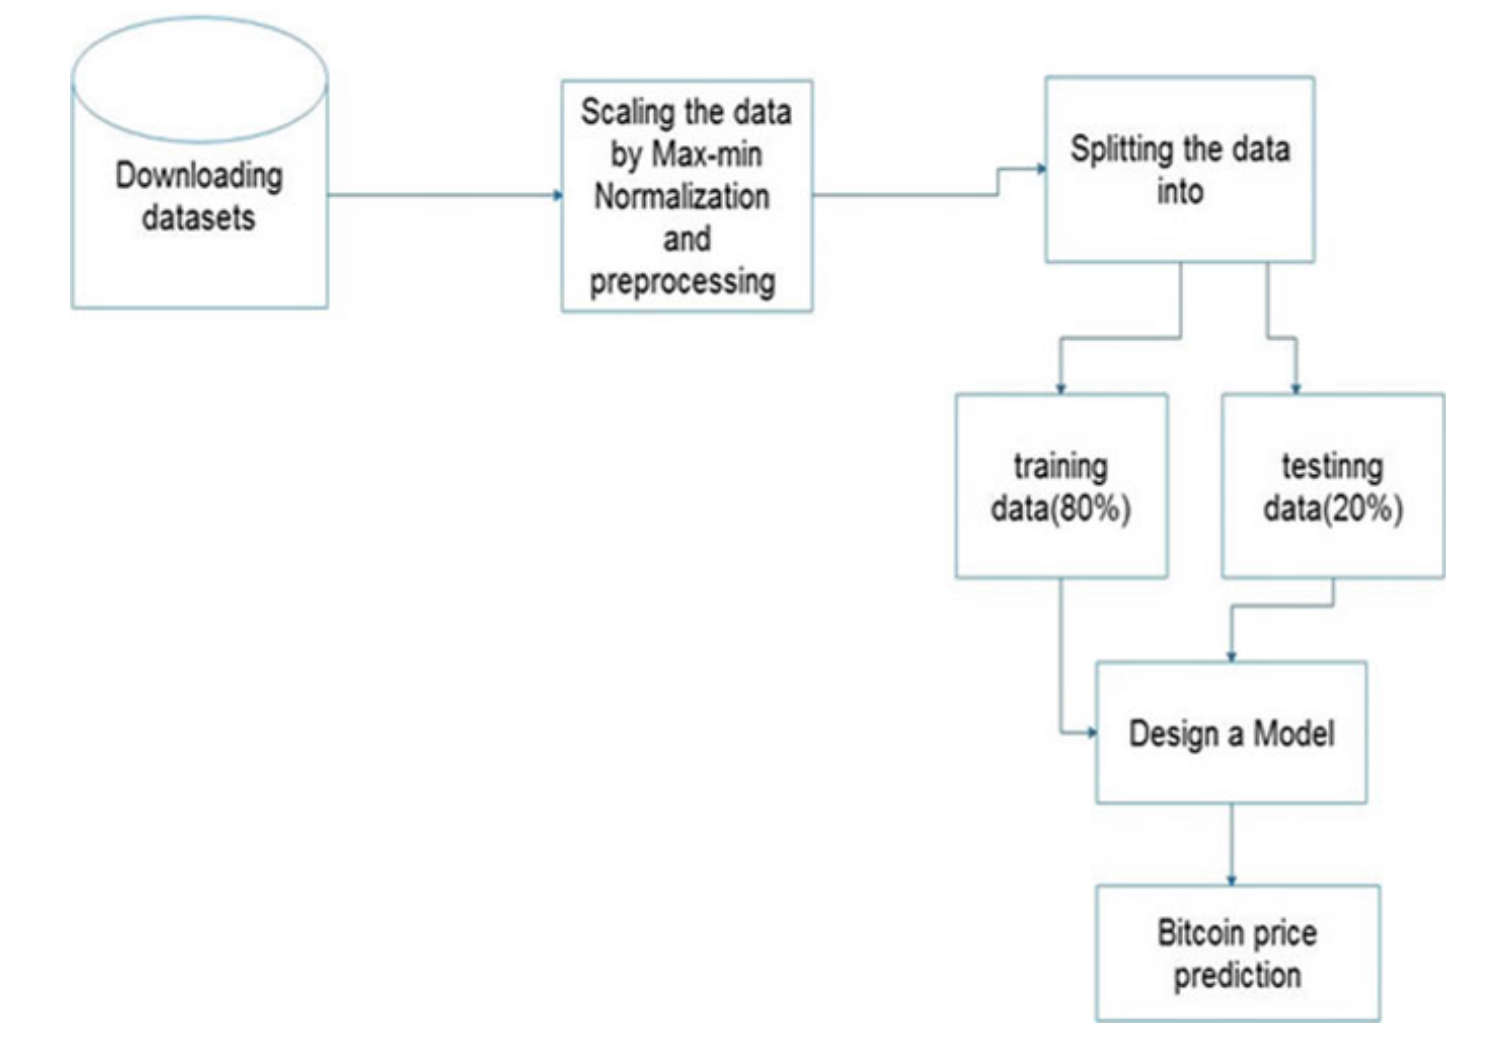
\includegraphics[width=\textwidth]{images/chapter5/flow.png}
    \caption{Luồng làm việc của bài báo}
    \label{fig:lstm_summary}
\end{figure}

\subsection{Kết quả}
Kết quả nghiên cứu cho thấy mô hình \textbf{GRU} có hiệu suất tốt hơn so với mô hình \textbf{LSTM} trong dự đoán ngắn hạn. Cụ thể, mô hình GRU đạt được độ chính xác cao hơn, với giá trị RMSE thấp hơn và thời gian hội tụ nhanh hơn so với LSTM. Kết quả được trình bày trong (Hình \ref{fig:hinh4}) cho thấy giá trị MSE của GRU giảm nhanh hơn và ổn định hơn trong quá trình huấn luyện so với LSTM.

Ngoài ra, các tác giả đã tiến hành đánh giá sự khác biệt giữa giá trị dự đoán và giá trị thực tế. (Hình \ref{fig:hinh5}) chỉ ra rằng sự khác biệt giữa giá trị thực tế và dự đoán của GRU ít hơn so với LSTM, đặc biệt là trong các khoảng thời gian ngắn.

\begin{figure}[h!]
    \centering
    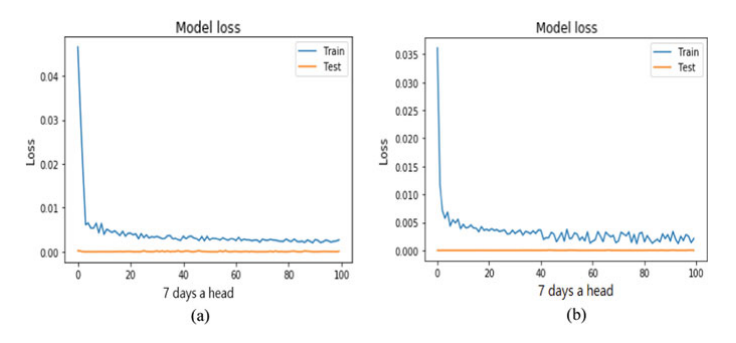
\includegraphics[width=\textwidth]{images/chapter5/hinh4.png}
    \caption{a. Biểu đồ MSE thu được từ mô hình LSTM b. Biểu đồ MSE thu được từ mô hình GRU}
    \label{fig:hinh4}
\end{figure}

\begin{figure}[h!]
    \centering
    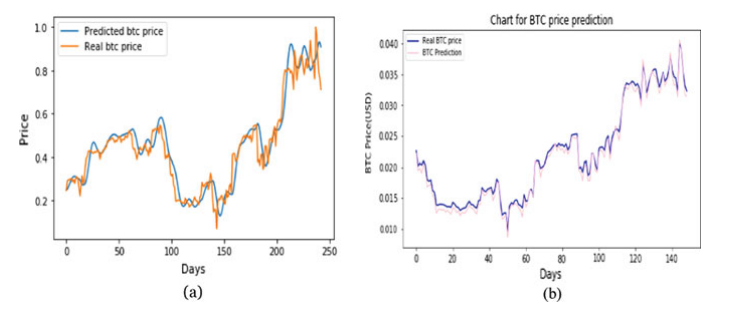
\includegraphics[width=\textwidth]{images/chapter5/hinh5.png}
    \caption{So sánh giá Bitcoin thực tế và dự đoán trong giai đoạn huấn luyện của LSTM (a) và GRU (b)}
    \label{fig:hinh5}
\end{figure}

\newpage

Tổng kết lại bài báo, họ chạy lại với nhiều window size và number of days ahead khác nhau, từ đó họ cung cấp được bảng kết quả sau: 
\textbf{Chú ý rằng kết quả RMSE và MAPE của họ có giá trị rất thấp do họ đã chuẩn hoá kết quả của họ.} 

\begin{figure}[h!]
    \centering
    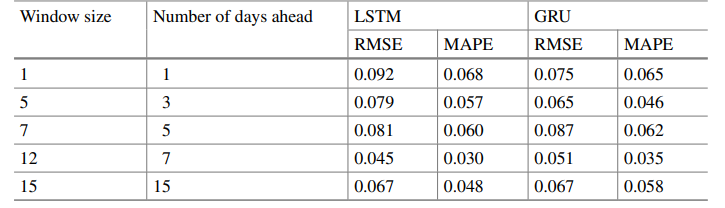
\includegraphics[width=\textwidth]{images/chapter5/res.png}
    \caption{So sánh giá trị RMSE và MAPE thu được từ các mô hình LSTM và GRU}
    \label{fig:res}
\end{figure}

Window size là số lượng bước thời gian trong quá khứ mà mô hình sẽ nhìn vào để dự đoán. Window size càng lớn, mô hình sẽ càng có nhiều thông tin lịch sử để dựa vào, điều này giúp mô hình phát hiện xu hướng tốt hơn nhưng cũng có thể dẫn đến việc mô hình trở nên phức tạp hơn và khó huấn luyện hơn.

Days ahead là số lượng ngày trong tương lai mà mô hình sẽ cố gắng dự đoán dựa trên dữ liệu quá khứ. Days ahead càng lớn, việc dự đoán sẽ càng khó khăn vì mô hình phải dự đoán nhiều ngày trong tương lai, điều này làm tăng độ không chắc chắn và có thể dẫn đến sai số lớn hơn.

\subsection{So sánh và đánh giá}
Nghiên cứu đã chỉ ra rằng \textbf{GRU} phù hợp hơn cho việc dự đoán giá Bitcoin trong ngắn hạn vì nó có thời gian hội tụ nhanh và độ chính xác cao hơn. Tuy nhiên, mô hình \textbf{LSTM} lại tỏ ra hiệu quả hơn trong các trường hợp dự đoán dài hạn, nơi cần học các phụ thuộc dài hạn của dữ liệu chuỗi thời gian.

Thực hiện một so sánh ngang với nghiên cứu cũng sử dụng đơn vị thời gian là ngày để dự đoán Bitcoin là bài báo gốc của chúng tôi, lỗi RMSE của hồi quy rừng ngẫu nhiên trong thí nghiệm trên sau khi chuẩn hoá như bên Awoke có kết quả 0,017 ở Giai đoạn 1 và 0,035 ở Giai đoạn 2 \textbf{tốt hơn} so với 0,045 của LSTM và 0,051 của GRU trong thí nghiệm của Awoke và cộng sự (2021) \cite{5}.

Lý do cho kết quả này có thể được giải thích đơn giản là mô hình của họ sử dụng cấu hình truyền thống và chưa được tinh chỉnh hoặc tích hợp các yếu tố nâng cao để cải thiện độ chính xác dự đoán. Trong khi đó, nghiên cứu của chúng tôi đã xem xét nhiều yếu tố đặc trưng hơn cho bài toán, chẳng hạn như giá của các đồng tiền điện tử khác hoặc giá vàng, đồng thời thực hiện tinh chỉnh tham số và cấu hình mô hình. Những điều này giúp kết quả của chúng tôi chính xác hơn.

Các tác giả cũng đề xuất rằng để cải thiện độ chính xác của các mô hình học sâu này, cần tích hợp thêm các yếu tố bên ngoài như hệ thống chính trị, quan hệ công chúng, và chính sách thị trường. Những yếu tố này có thể ảnh hưởng mạnh mẽ đến sự biến động giá của tiền điện tử và có thể giúp nâng cao hiệu quả của các mô hình dự đoán.

\section{Forecasting the price of Bitcoin using deep learning}
\subsection{Giới thiệu bài báo}
Bài báo này được thực hiện bởi nhóm tác giả Mingxi Liu và cộng sự xuất bản năm 2021. Mục tiêu của bài báo là xây dựng một mô hình dự đoán giá Bitcoin dựa trên các yếu tố ảnh hưởng từ thị trường tiền điện tử, sự quan tâm của công chúng, và môi trường kinh tế vĩ mô. Để đạt được mục đích này, nhóm tác giả đã sử dụng phương pháp học sâu, cụ thể là mô hình \textbf{Stacked Denoising Autoencoders (SDAE)}, để dự đoán giá của Bitcoin và so sánh hiệu suất của mô hình này với các mô hình học máy truyền thống khác như Mạng Nơ-ron Truyền ngược (BPNN) và Hồi quy Vector Hỗ trợ (SVR). 

Bài báo này giới thiệu và cung cấp một số phương pháp và mô hình học sâu tiên tiến để dự đoán giá Bitcoin, tạo nên cơ sở so sánh đáng giá với mô hình trong bài báo gốc của chúng tôi.
\subsection{Bộ dữ liệu}
\textbf{Xử lý dữ liệu}
Giai đoạn xử lý dữ liệu rất quan trọng để đảm bảo chất lượng và độ tin cậy của dữ liệu đầu vào được sử dụng để huấn luyện mô hình SDAE. Các bước sau đã được thực hiện:

\begin{enumerate}
    \item \textbf{Thu thập dữ liệu}: Dữ liệu được sử dụng trong nghiên cứu này được thu thập từ nhiều nguồn khác nhau, bao gồm các trang web giao dịch Bitcoin chuyên nghiệp như `www.coindesk.com` và `BTC.com`. Dữ liệu được thu thập từ tháng 7 năm 2013 đến tháng 12 năm 2019, bao gồm các yếu tố ảnh hưởng đến giá Bitcoin.
    
    \item \textbf{Lựa chọn đặc trưng}: Tổng cộng có 40 yếu tố quyết định đã được xác định, chia thành ba nhóm:
    \begin{itemize}
        \item \textbf{Thị trường tiền điện tử}: Bao gồm khối lượng giao dịch hàng ngày của Bitcoin, vốn hóa thị trường, hashrate, v.v.
        \item \textbf{Sự quan tâm của công chúng}: Được đo lường bằng khối lượng tìm kiếm từ các công cụ tìm kiếm khác nhau như Google và Baidu.
        \item \textbf{Môi trường kinh tế vĩ mô}: Bao gồm các chỉ số thị trường chứng khoán, giá dầu thô, tỷ giá hối đoái, v.v.
    \end{itemize}
    
    \item \textbf{Làm sạch dữ liệu}: Các giá trị bị thiếu đã được loại bỏ và dữ liệu được lọc để đảm bảo tính nhất quán. Chỉ các điểm dữ liệu có đầy đủ thông tin cho tất cả 40 yếu tố mới được giữ lại, kết quả là một tập dữ liệu gồm 1356 ngày.
    
    \item \textbf{Chuẩn hóa}: Tất cả dữ liệu đều được chuẩn hóa về khoảng $[0, 1]$ để loại bỏ tác động của các thang đo khác nhau giữa các đặc trưng. Bước này rất quan trọng để cải thiện sự ổn định và hội tụ của quá trình huấn luyện mạng nơ-ron.
\end{enumerate}

\begin{figure}[h!]
    \centering
    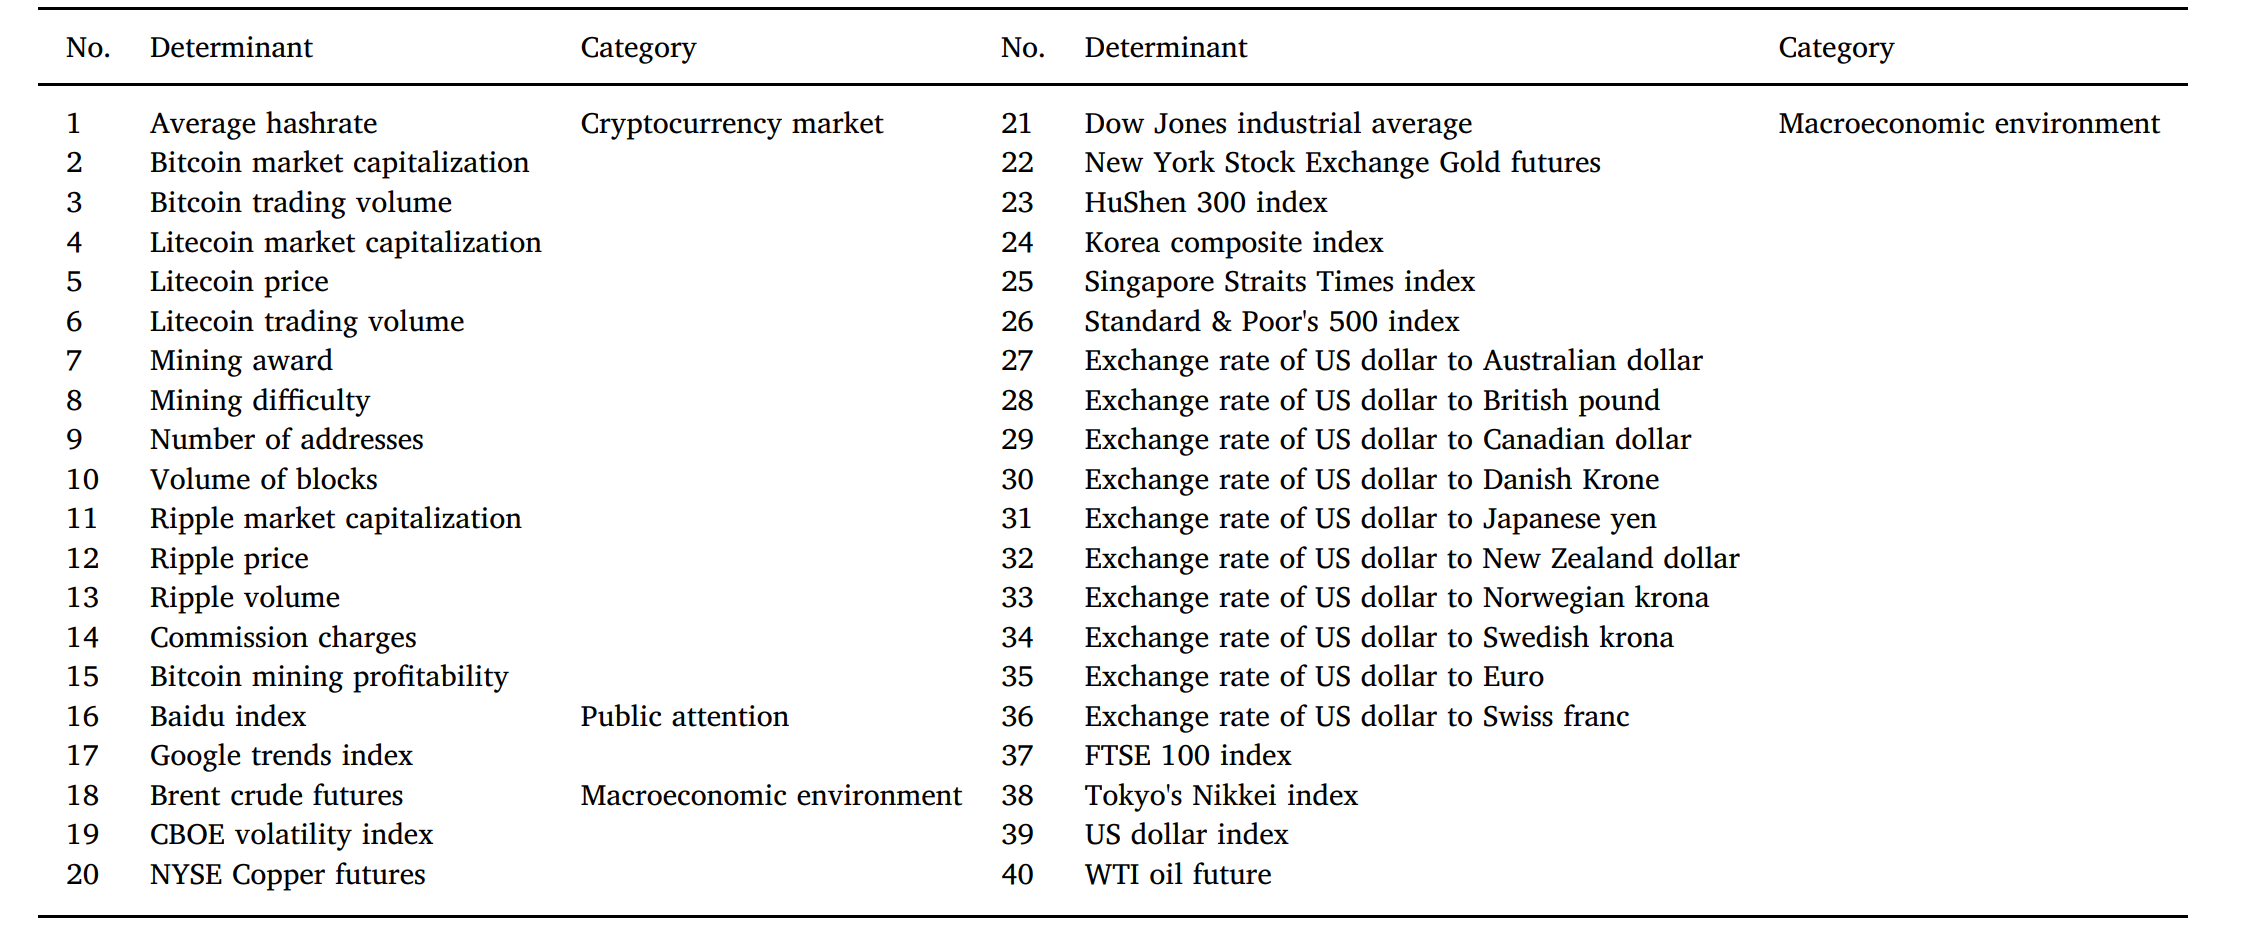
\includegraphics[width=\textwidth]{images/chapter5/feature.png}
    \caption{Danh sách đặc trưng của mô hình}
    \label{fig:feature}
\end{figure}

\newpage

\subsection{Phương pháp}
Stacked Denoising Autoencoders (SDAE) là một mô hình học sâu phổ biến nhờ vào khả năng dự đoán vượt trội của nó. SDAE được xây dựng dựa trên việc xếp chồng các lớp Denoising Autoencoders (DAE). Để hiểu rõ về DAE, trước hết ta cần đi qua về Autoencoder (AE).


\textbf{Autoencoder (AE)} là một mạng nơ-ron được thiết kế để học các biểu diễn hiệu quả của dữ liệu, thường được sử dụng để giảm số chiều. Nó bao gồm một \textbf{bộ mã hóa} và một \textbf{bộ giải mã}.

\textbf{Bộ mã hóa:} ánh xạ vector đầu vào $\mathbf{x} \in [0, 1]^d$ thành biểu diễn ẩn $\mathbf{y} \in [0, 1]^{d'}$ bằng phương trình sau:

\begin{equation}
    \mathbf{y} = f_\theta(\mathbf{x}) = s(\mathbf{W} \mathbf{x} + \mathbf{b})
\end{equation}

với $s(\cdot)$ là hàm kích hoạt (ví dụ: sigmoid), $\mathbf{W}$ là ma trận trọng số có kích thước $d' \times d$, và $\mathbf{b}$ là vector bù có kích thước $d'$.

\textbf{Bộ giải mã:} tái tạo lại vector đầu vào $\mathbf{z} \in [0, 1]^d$ từ biểu diễn ẩn $\mathbf{y}$ như sau:

\begin{equation}
    \mathbf{z} = g_{\theta'}(\mathbf{y}) = s'(\mathbf{W'} \mathbf{y} + \mathbf{b'})
\end{equation}

với $s'(\cdot)$ là một hàm kích hoạt khác (ví dụ: hàm tuyến tính), và $\mathbf{W'}$ và $\mathbf{b'}$ là trọng số và bù của bộ giải mã.

Quá trình huấn luyện nhằm mục tiêu tối thiểu hóa sai số tái tạo giữa đầu vào $\mathbf{x}$ và đầu ra tái tạo $\mathbf{z}$. Hàm mất mát $L$ được định nghĩa như sau:

\begin{equation}
    L(\mathbf{x}, \mathbf{z}) = \frac{1}{n} \sum_{i=1}^n \left( \mathbf{x}^{(i)} - \mathbf{z}^{(i)} \right)^2
\end{equation}


\textbf{Denoising Autoencoder (DAE)} là một biến thể của AE, học cách tái tạo đầu vào từ một phiên bản bị nhiễu. Đầu vào $\mathbf{x}$ bị làm nhiễu thành $\tilde{\mathbf{x}}$ bằng cách thêm nhiễu, và mô hình học cách ánh xạ $\tilde{\mathbf{x}}$ trở lại thành $\mathbf{x}$ ban đầu. Mục tiêu là tối thiểu hóa sai số tái tạo giữa $\mathbf{x}$ và đầu ra $\mathbf{z}$:

\begin{equation}
    L(\mathbf{x}, \mathbf{z}) = \frac{1}{n} \sum_{i=1}^n \left( \mathbf{x}^{(i)} - g_{\theta'}(f_\theta(\tilde{\mathbf{x}}^{(i)})) \right)^2
\end{equation}

\begin{figure}[h!]
    \centering
    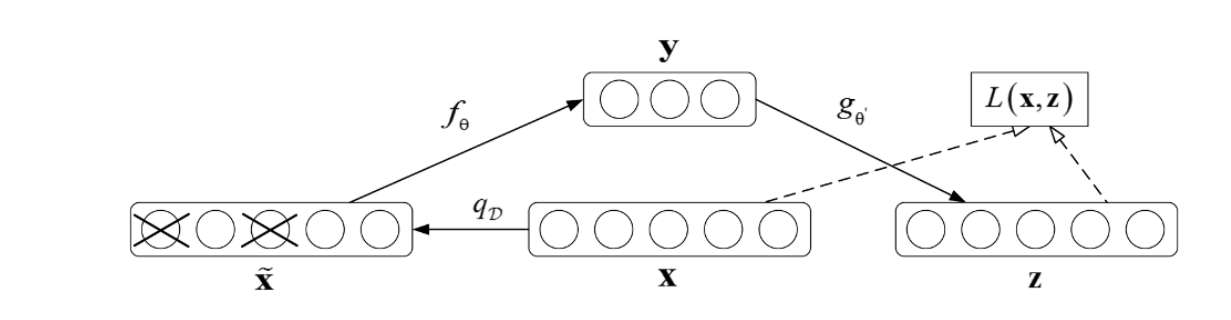
\includegraphics[width=\textwidth]{images/chapter5/de.png}
    \caption{Kiến trúc của Denoising Autoencoder}
    \label{fig:dae}
\end{figure}

\textbf{Stacked Denoising Autoencoder (SDAE)} được xây dựng bằng cách chồng nhiều DAE lên nhau, trong đó đầu ra của mỗi lớp được sử dụng làm đầu vào cho lớp tiếp theo. Kiến trúc sâu này cho phép mô hình học các đặc trưng phân cấp từ dữ liệu.

\textbf{Quá trình huấn luyện}
Quá trình huấn luyện SDAE bao gồm hai bước chính:

\begin{enumerate}
    \item \textbf{Huấn luyện không giám sát}: Mỗi lớp của SDAE được huấn luyện như một DAE theo cách không giám sát để học biểu diễn tốt của dữ liệu đầu vào. Điều này giúp khởi tạo hiệu quả các tham số của mạng.
    
    \item \textbf{Tinh chỉnh có giám sát}: Sau khi huấn luyện không giám sát, toàn bộ mạng được tinh chỉnh bằng cách sử dụng dữ liệu có nhãn để tối thiểu hóa sai số dự đoán. Mục tiêu là tối ưu hóa các tham số cho bài toán dự đoán.
\end{enumerate}

\textbf{Tối ưu hóa siêu tham số}
Việc tối ưu hóa các siêu tham số là rất quan trọng để cải thiện hiệu suất của mô hình SDAE. Các siêu tham số của mô hình được xác định thông qua quá trình thử nghiệm và tham khảo từ các nghiên cứu trước. Cụ thể, cấu trúc mạng của SDAE được thiết lập như sau:

\begin{itemize}
    \item \textbf{Cấu trúc mạng}: [40, 40, 20, 1] - bao gồm ba lớp ẩn và một lớp đầu ra.
    \item \textbf{Hàm kích hoạt}: Hàm sigmoid được sử dụng cho các lớp mã hóa và hàm tuyến tính cho lớp giải mã.
    \item \textbf{Tốc độ học (learning rate)}: 0.1 - được sử dụng để điều chỉnh mức độ thay đổi của trọng số trong quá trình huấn luyện.
    \item \textbf{Kích thước lô (batch size)}: 50 - số lượng mẫu trong mỗi lần cập nhật trọng số.
    \item \textbf{Số epoch}: 20 - số lần toàn bộ tập dữ liệu được huấn luyện qua mô hình.
\end{itemize}

\textbf{Đánh giá mô hình}
Hiệu suất của mô hình SDAE được so sánh với các mô hình truyền thống như Mạng Nơ-ron Truyền ngược (BPNN) và Hồi quy Vector Hỗ trợ (SVR) bằng các chỉ số sau:

\begin{itemize}
    \item \textbf{Sai số phần trăm trung bình tuyệt đối (MAPE)}:
    \begin{equation}
        \text{MAPE} = \frac{1}{m} \sum_{t=1}^m \left| \frac{y(t) - \hat{y}(t)}{y(t)} \right|
    \end{equation}
    
    \item \textbf{Căn bậc hai của sai số bình phương trung bình (RMSE)}:
    \begin{equation}
        \text{RMSE} = \sqrt{\frac{1}{m} \sum_{t=1}^m \left( y(t) - \hat{y}(t) \right)^2}
    \end{equation}
    
    \item \textbf{Độ chính xác hướng (DA)}:
    \begin{equation}
        \text{DA} = \frac{1}{m} \sum_{t=1}^m a(t) \times 100\%
    \end{equation}
    với $a(t) = 1$ nếu hướng dự đoán trùng khớp với hướng thực tế, ngược lại $a(t) = 0$.
\end{itemize}
\subsection{Kết quả}

Kết quả dự đoán của các mô hình khác nhau được trình bày trong Bảng \ref{table:results}.

\begin{table}[h]
    \centering
    \begin{tabular}{|l|c|c|c|}
        \hline
        \textbf{Mô hình} & \textbf{MAPE} & \textbf{RMSE} & \textbf{DA} \\
        \hline
        BPNN & 0.3736 & 390.07 & 0.5457 \\
        PCA-SVR & 0.2278 & 318.62 & 0.5728 \\
        SVR & 0.1783 & 248.24 & 0.5750 \\
        SDAE & \textbf{0.1019} & \textbf{160.63} & \textbf{0.5985} \\
        \hline
    \end{tabular}
    \caption{Kết quả dự đoán giá Bitcoin của các mô hình khác nhau.}
    \label{table:results}
\end{table}

Nghiên cứu này đã sử dụng mô hình học sâu Stacked Denoising Autoencoders (SDAE) để dự đoán giá Bitcoin và so sánh với các mô hình truyền thống như BPNN và SVR. Kết quả cho thấy SDAE vượt trội về cả sai số dự đoán và độ chính xác hướng, nhờ khả năng học các đặc trưng phân cấp từ dữ liệu, giúp cải thiện dự đoán trong bối cảnh thị trường tiền điện tử biến động mạnh. Những phát hiện này không chỉ hỗ trợ nhà đầu tư mà còn cung cấp cơ sở cho các cơ quan chính phủ trong việc xây dựng chính sách quản lý liên quan đến tiền điện tử. Mô hình SDAE còn có tiềm năng mở rộng để dự đoán các loại tiền điện tử khác, góp phần quản lý rủi ro và hỗ trợ quyết định hiệu quả.
\subsection{So sánh và đánh giá}

Thực hiện một so sánh ngang với nghiên cứu cũng sử dụng đơn vị thời gian là ngày để dự đoán Bitcoin là bài báo gốc của chúng tôi, lỗi RMSE của hồi quy rừng ngẫu nhiên trong thí nghiệm trên sau khi \textbf{chuẩn hoá} có kết quả 0,017 ở Giai đoạn 1 và 0,035 ở Giai đoạn 2 \textbf{tệ hơn} so với 0.009 của SDAE trong thí nghiệm của Mingxi Liu và cộng sự (2021) \cite{6} cũng đã được \textbf{chuẩn hoá} kết quả tương tự.

Trong bài báo này, SDAE hoạt động hiệu quả nhờ khả năng học các đặc trưng từ dữ liệu có nhiễu. Sử dụng kiến trúc Denoising Autoencoder, SDAE có thể loại bỏ nhiễu và trích xuất các đặc trưng tiềm ẩn từ dữ liệu thô, từ đó cải thiện khả năng khái quát hóa và tăng độ chính xác trong dự đoán giá Bitcoin.

SDAE có khả năng học các đặc trưng phân cấp từ dữ liệu, điều này đặc biệt quan trọng khi làm việc với các yếu tố quyết định phức tạp và phi tuyến trong thị trường tiền điện tử. Mỗi lớp Denoising Autoencoder học một mức độ trừu tượng khác nhau, giúp mô hình nắm bắt được mối quan hệ phức tạp giữa các yếu tố kinh tế, thị trường, và công chúng, qua đó nâng cao hiệu suất dự đoán.

Cuối cùng, việc tác giả xử lý dữ liệu kỹ lưỡng bằng cách trích xuất đặc trưng từ nhiều yếu tố liên quan, kết hợp với tối ưu hóa hiệu quả các siêu tham số, chính là lý do tại sao kết quả của họ có độ chính xác vượt trội hơn so với bài báo gốc mà chúng tôi đã trình bày.
